\subsection{Household Average Responses to Time-Of-Use Electricity Pricing}
\label{Subsection:Household-Average-Responses-to-Time-Of-Use-Electricity-Pricing}

\subsubsection{Half-hourly Average Treatment Effects}
\label{Sub-subsection:Half-hourly-Average-Treatment-Effects}
Utilizing a panel DID identification strategy, I first measure the impact of the TOU prices on 30-minute-interval household electricity consumption. To obtain the Average Treatment Effect (ATE) for each half-hour interval, I estimate the following specification:
\begin{equation}
\small
\begin{split}
    \textit{kWh}_{itw} \ 
    & = \ \beta_{w} \mathbb{1}\big[ \text{Treatment \& Post} \big]_{it} \ + \ \alpha_{iw} \ + \ \gamma_{tw} \ + \ \delta_{m} \ + \ \epsilon_{itw}
\end{split}
\label{Eq:Model-Specification_Half-Hourly-Average-Treatment-Effects}
\end{equation}
The term $kWh_{itw}$ is the electricity consumption by household $i$ on the day $t$ during the half-hourly time window $w$. The indicator variable $\mathbb{1}\big[ \text{Treatment \& Post} \big]_{it}$ is equal to 1 only if household $i$ is in the treatment group and the day $t$ is in the treatment period. The terms $\alpha_{iw}$, $\gamma_{tw}$, and $\delta_{m}$ are household-by-half-hourly-interval, day-of-sample-by-half-hourly-time-window, and month-of-year fixed effects, respectively. In the specification, the point estimates of $\beta_{w}$, representing the ATE for each 30-minute interval $w$, are the parameters of interest. I cluster the standard errors at the household and the day of experiment levels to correct for serial correlation.

\afterpage{
    \begin{figure}
        \centering
        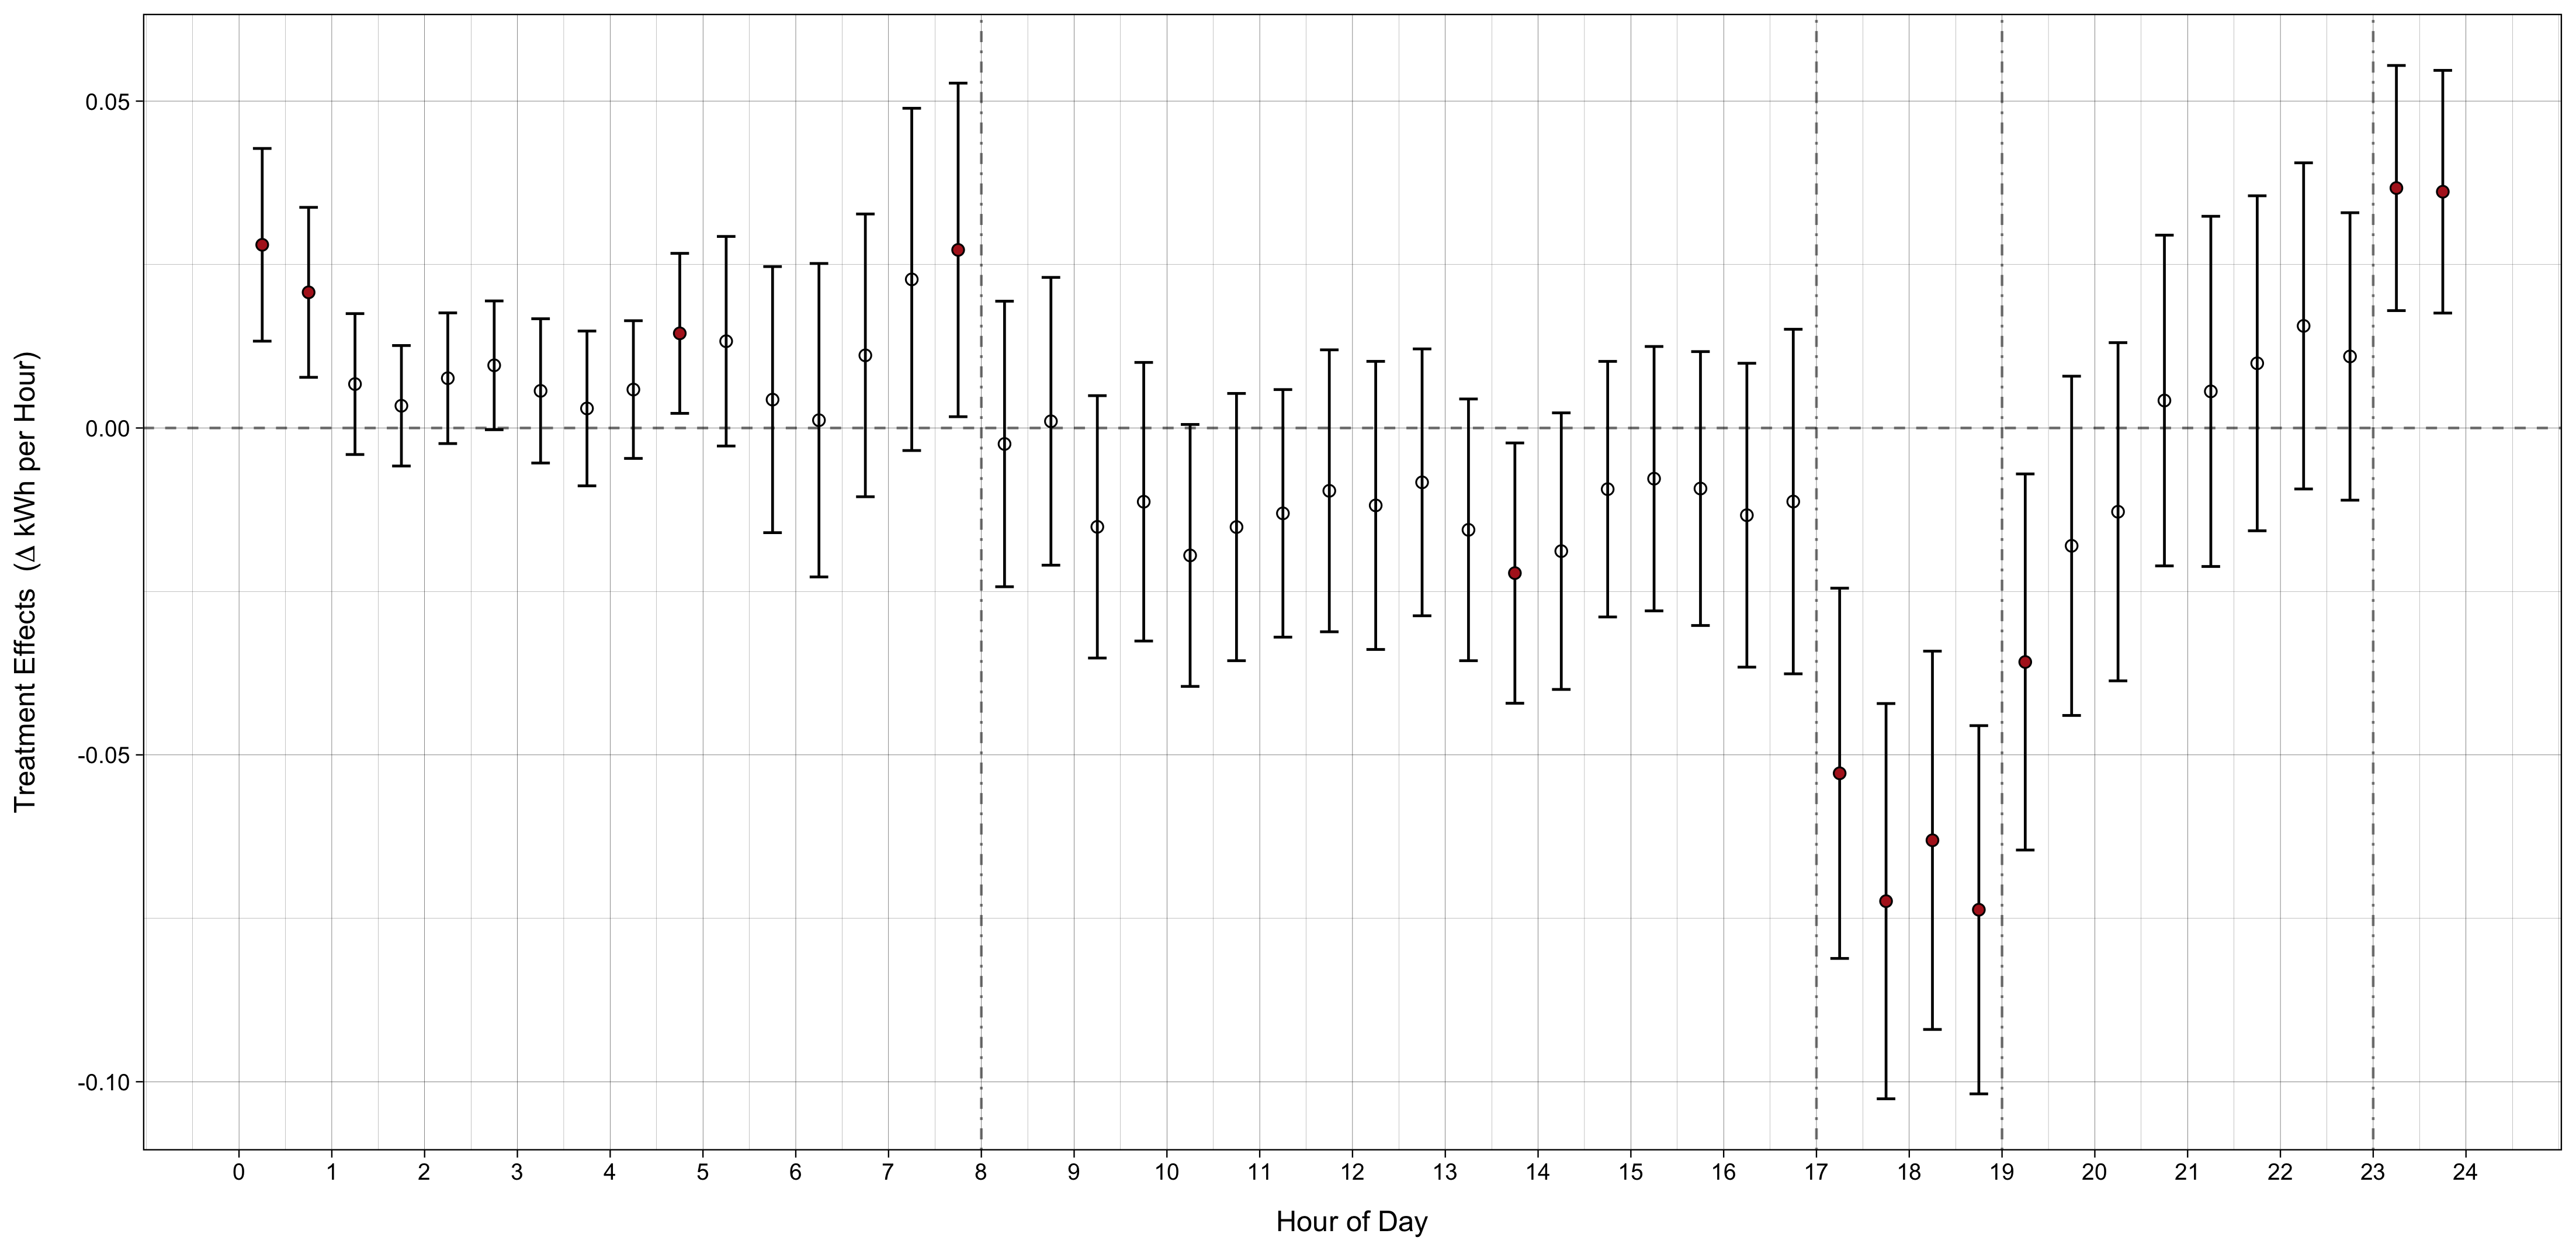
\includegraphics[scale = 0.09]{03_Chapter-2/00A_Figures/Figure_Time-Profile-of-Half-Hourly-ATEs.png}
        \caption{Half-hourly Average Treatment Effects}
        \caption*{
            {\small
            \textit{Note}: This figure depicts the time profile of half-hourly average treatment effects with 95\% confidence intervals. Standard errors are clustered at the household and date levels to adjust for serial correlation. As clearly illustrated, the treated households significantly reduced their electricity consumption during peak hours. A more interesting phenomenon is that they reduced their electricity consumption in hours leading up to and following the peak rate period, during which the applicable unit rate was lower than the flat rate in the baseline period, even though most of the estimated treatment effects are statistically insignificant in those hours. 
        }}
        \label{Figure:Half-Hourly-Average-Treatment-Effects}
    \end{figure}
}
Figure \ref{Figure:Half-Hourly-Average-Treatment-Effects} summarizes the estimated ATEs in the form of a time profile. As already demonstrated in \cite{Peaking-Interest:How-Awareness-Drives-the-Effectiveness-of-Time-of-Use-Electricity-Pricing_Prest_2020}, peak hours (i.e., from 5:00 p.m. to 7:00 p.m.) show dominant electricity savings. The figure also demonstrates reductions in household electricity consumption not only in most of the meter readings prior to the peak rate period but also in three successive meter readings right after the period, even though the reductions, with two exceptions, are not statistically significant. The insignificant reductions in household electricity consumption are interesting because TOU prices in off-peak hours (i.e., prices in the night and day rate periods) were lower than the flat rate in the baseline period. The counterintuitive changes might indicate that households preemptively adjusted their consumption behavior to avoid the incident of paying higher prices. In other words, the peak-hour price increases under the TOU program were likely to cause some spillover effects in the hours leading up to and following the peak rate period. To explore whether households responded to the TOU program outside of the peak rate period as well or not, in the following empirical analysis, I will also pay attention to the off-peak hours, particularly the hours surrounding the peak rate period.


\subsubsection{Hourly Average Treatment Effects in and near the Peak Rate Period}
\label{Sub-subsection:Hourly-Average-Treatment-Effects-in-and-near-the-Peak-Rate-Period}
Estimating by-tariff-group ATEs in and near the peak rate period allows understanding how the relationship between the degree of change in household electricity consumption and the magnitude of a peak-demand-hour price increase evolves in and near the peak rate period.\footnote{In this paper, the effects of four different information stimuli on household electricity consumption are not of interest. \cite{The-Effect-of-Information-on-TOU-Electricity-Use:An-Irish-Residential-Study_Pon_2017} studied the effects in detail using the same datasets.} To do so, I run the following regression for each of the four tariff groups:
\begin{equation}
\small
    \textit{kWh}_{ith} \ 
     = \ \beta_{p} \mathbb{1}\big[ \text{Treatment \& Post} \big]_{it} \ + \ \alpha_{iw} \ + \ \gamma_{tw} \ + \ \delta_{m} \ + \ \epsilon_{ith}
\label{Eq:Model-Specification_Hourly-Average-Treatment-Effects}
\end{equation}

Excepting the dependent variable and the parameter of interest, the econometric model above is the same as (\ref{Eq:Model-Specification_Half-Hourly-Average-Treatment-Effects}). Specifically, the response variable $kWh_{ith}$, which means the electricity consumption by household $i$ on the day $t$ during the hour of the day $h$, is utilized due to its better accessibility in interpretation. The point estimates of $\beta_{p}$ indicate the ATE for each of the three intervals included in rate period $p$. Table \ref{Table:Hourly-Average-Treatment-Effects-in-and-near-the-Peak-Rate-Period} summarizes the regression results.
\begin{landscape}
    \afterpage{
    \begin{sidewaystable}[t!]
        \centering
        \caption{Hourly Average Treatment Effects in and near the Peak Rate Period}
        \label{Table:Hourly-Average-Treatment-Effects-in-and-near-the-Peak-Rate-Period}
        \small
        \begin{adjustbox}{scale = 0.65}
            \begin{threeparttable}
                \begin{tabular}{@{\extracolsep{1pt}}lccccccccccccccc}
                    \\[-5.5ex]
                    \hline \hline
                    \\[-3.0ex]
%                    & \multicolumn{15}{c}{Dependent Variable} \\
%                    \\[-3.0ex]
%                    \cline{2-16}
%                    \\[-3.0ex]
                    & \multicolumn{15}{c}{Hourly Electricity Consumption  (kWh/Hour)} \\
                    \\[-3.0ex]
                    & (1) & (2) & (3) & (4) & (5) & (6) & (7) & (8) & (9) & (10) & (11) & (12) & (13) & (14) & (15)\\
                    \\[-3.0ex]
                    \hline
                    \\[-2.0ex]
                    $\mathbb{1}$[Treatment \& Post] & $-$0.048$^{***}$ & $-$0.053$^{*}$ & $-$0.002 & $-$0.049 & $-$0.032$^{***}$ & $-$0.125$^{***}$ & $-$0.161$^{***}$ & $-$0.119$^{***}$ & $-$0.249$^{***}$ & $-$0.143$^{***}$ & $-$0.082$^{***}$ & $-$0.055$^{*}$ & $-$0.015 & $-$0.113$^{**}$ & $-$0.058$^{***}$ \\
                    & (0.016) & (0.027) & (0.017) & (0.031) & (0.011) & (0.020) & (0.036) & (0.022) & (0.044) & (0.015) & (0.020) & (0.030) & (0.021) & (0.048) & (0.015) \\
                    & & & & & & & & & & & & & & & \\
                    \hline
                    \\[-2.0ex]
                    Description of Interval & Pre-Peak & Pre-Peak & Pre-Peak & Pre-Peak & Pre-Peak & Peak & Peak & Peak & Peak & Peak & Post-Peak & Post-Peak & Post-Peak & Post-Peak & Post-Peak \\
                    Interval of Hours & 15 to 16 & 15 to 16 & 15 to 16 & 15 to 16 & 15 to 16 & 17 to 18 & 17 to 18 & 17 to 18 & 17 to 18 & 17 to 18 & 19 to 20 & 19 to 20 & 19 to 20 & 19 to 20 & 19 to 20 \\
                    Tariff Group & A & B & C & D & All & A & B & C & D & All & A & B & C & D & All \\
                    FEs: Household by Half-Hourly Time Window & Yes & Yes & Yes & Yes & Yes & Yes & Yes & Yes & Yes & Yes & Yes & Yes & Yes & Yes & Yes \\
                    FEs: Day of Week by Half-Hourly Time Window & Yes & Yes & Yes & Yes & Yes & Yes & Yes & Yes & Yes & Yes & Yes & Yes & Yes & Yes & Yes \\
                    FEs: Month of Year & Yes & Yes & Yes & Yes & Yes & Yes & Yes & Yes & Yes & Yes & Yes & Yes & Yes & Yes & Yes \\
                    Observations & 506,540 & 326,800 & 511,700 & 331,960 & 1,006,200 & 506,540 & 326,800 & 511,700 & 331,960 & 1,006,200 & 506,540 & 326,800 & 511,700 & 331,960 & 1,006,200 \\
                    Adjusted R$^{2}$ & 0.312 & 0.330 & 0.320 & 0.327 & 0.308 & 0.384 & 0.397 & 0.383 & 0.367 & 0.379 & 0.371 & 0.389 & 0.376 & 0.361 & 0.372 \\
                    \\[-2.0ex]
                    \hline \hline
                    \\[-4.5ex]
                \end{tabular}
                \begin{tablenotes}[flushleft]
                    \footnotesize
                    \item \textit{Note}: * $p < 0.1$, ** $p < 0.05$, and *** $p < 0.01$.
                \end{tablenotes}
            \end{threeparttable}
        \end{adjustbox}
    \end{sidewaystable}
}

\end{landscape}

The measured ATEs for the peak rate period re-confirm the finding provided in \cite{Peaking-Interest:How-Awareness-Drives-the-Effectiveness-of-Time-of-Use-Electricity-Pricing_Prest_2020}.\footnote{See Figure 6 in \cite{Peaking-Interest:How-Awareness-Drives-the-Effectiveness-of-Time-of-Use-Electricity-Pricing_Prest_2020}.} The table clearly shows that within-household aggregate demand for electricity during the peak rate period declined, with a significance level of 0.01, due to the deployment of TOU pricing. However, based on the point estimates for the four tariff groups, it is unclear whether an incremental change in peak-rate-period price increase induces a statistically meaningful additional change in household electricity consumption or not. 

To quantify how residential consumers responded to the TOU program in off-peak hours close to the peak rate period, I also estimate ATEs in periods of two hours before and after the peak rate period (i.e., in pre- and post-peak periods). Interestingly, the table also demonstrates that in the pre- and post-peak periods, the implementation of the TOU tariff structures resulted in reductions in household electricity consumption, which are statistically different from zero, even though TOU prices were lower than the flat rate of 14.1 cents per kWh.\footnote{Even insignificant point estimates (i.e., point estimates for Tariff Groups C and D in the pre-peak interval and Tariff Group C in the post-peak interval) have negative values.} The reductions in both periods surrounding the peak hours suggest that the impact of the price increases in the peak rate period overtook the impact of the price drops in each off-peak period. Therefore, in the following empirical analysis, I will focus on linking household electricity consumption in the pre- and post-peak periods with the price increases in the peak rate period, instead of the price decreases in those off-peak periods. 



\subsection{Breakdown of Household Responses to Time-Of-Use Electricity Pricing}
\label{Subsection:Breakdown-of-Responses-to-Time-Of-Use-Electricity-Pricing}

\subsubsection{Breakdown of Household Responses in and near the Peak Rate Period}
\label{Sub-subsection:Breakdown-of-Household-Responses-in-and-near-the-Peak-Rate-Period}
\afterpage{
    \begin{figure}[t!]
        \centering
        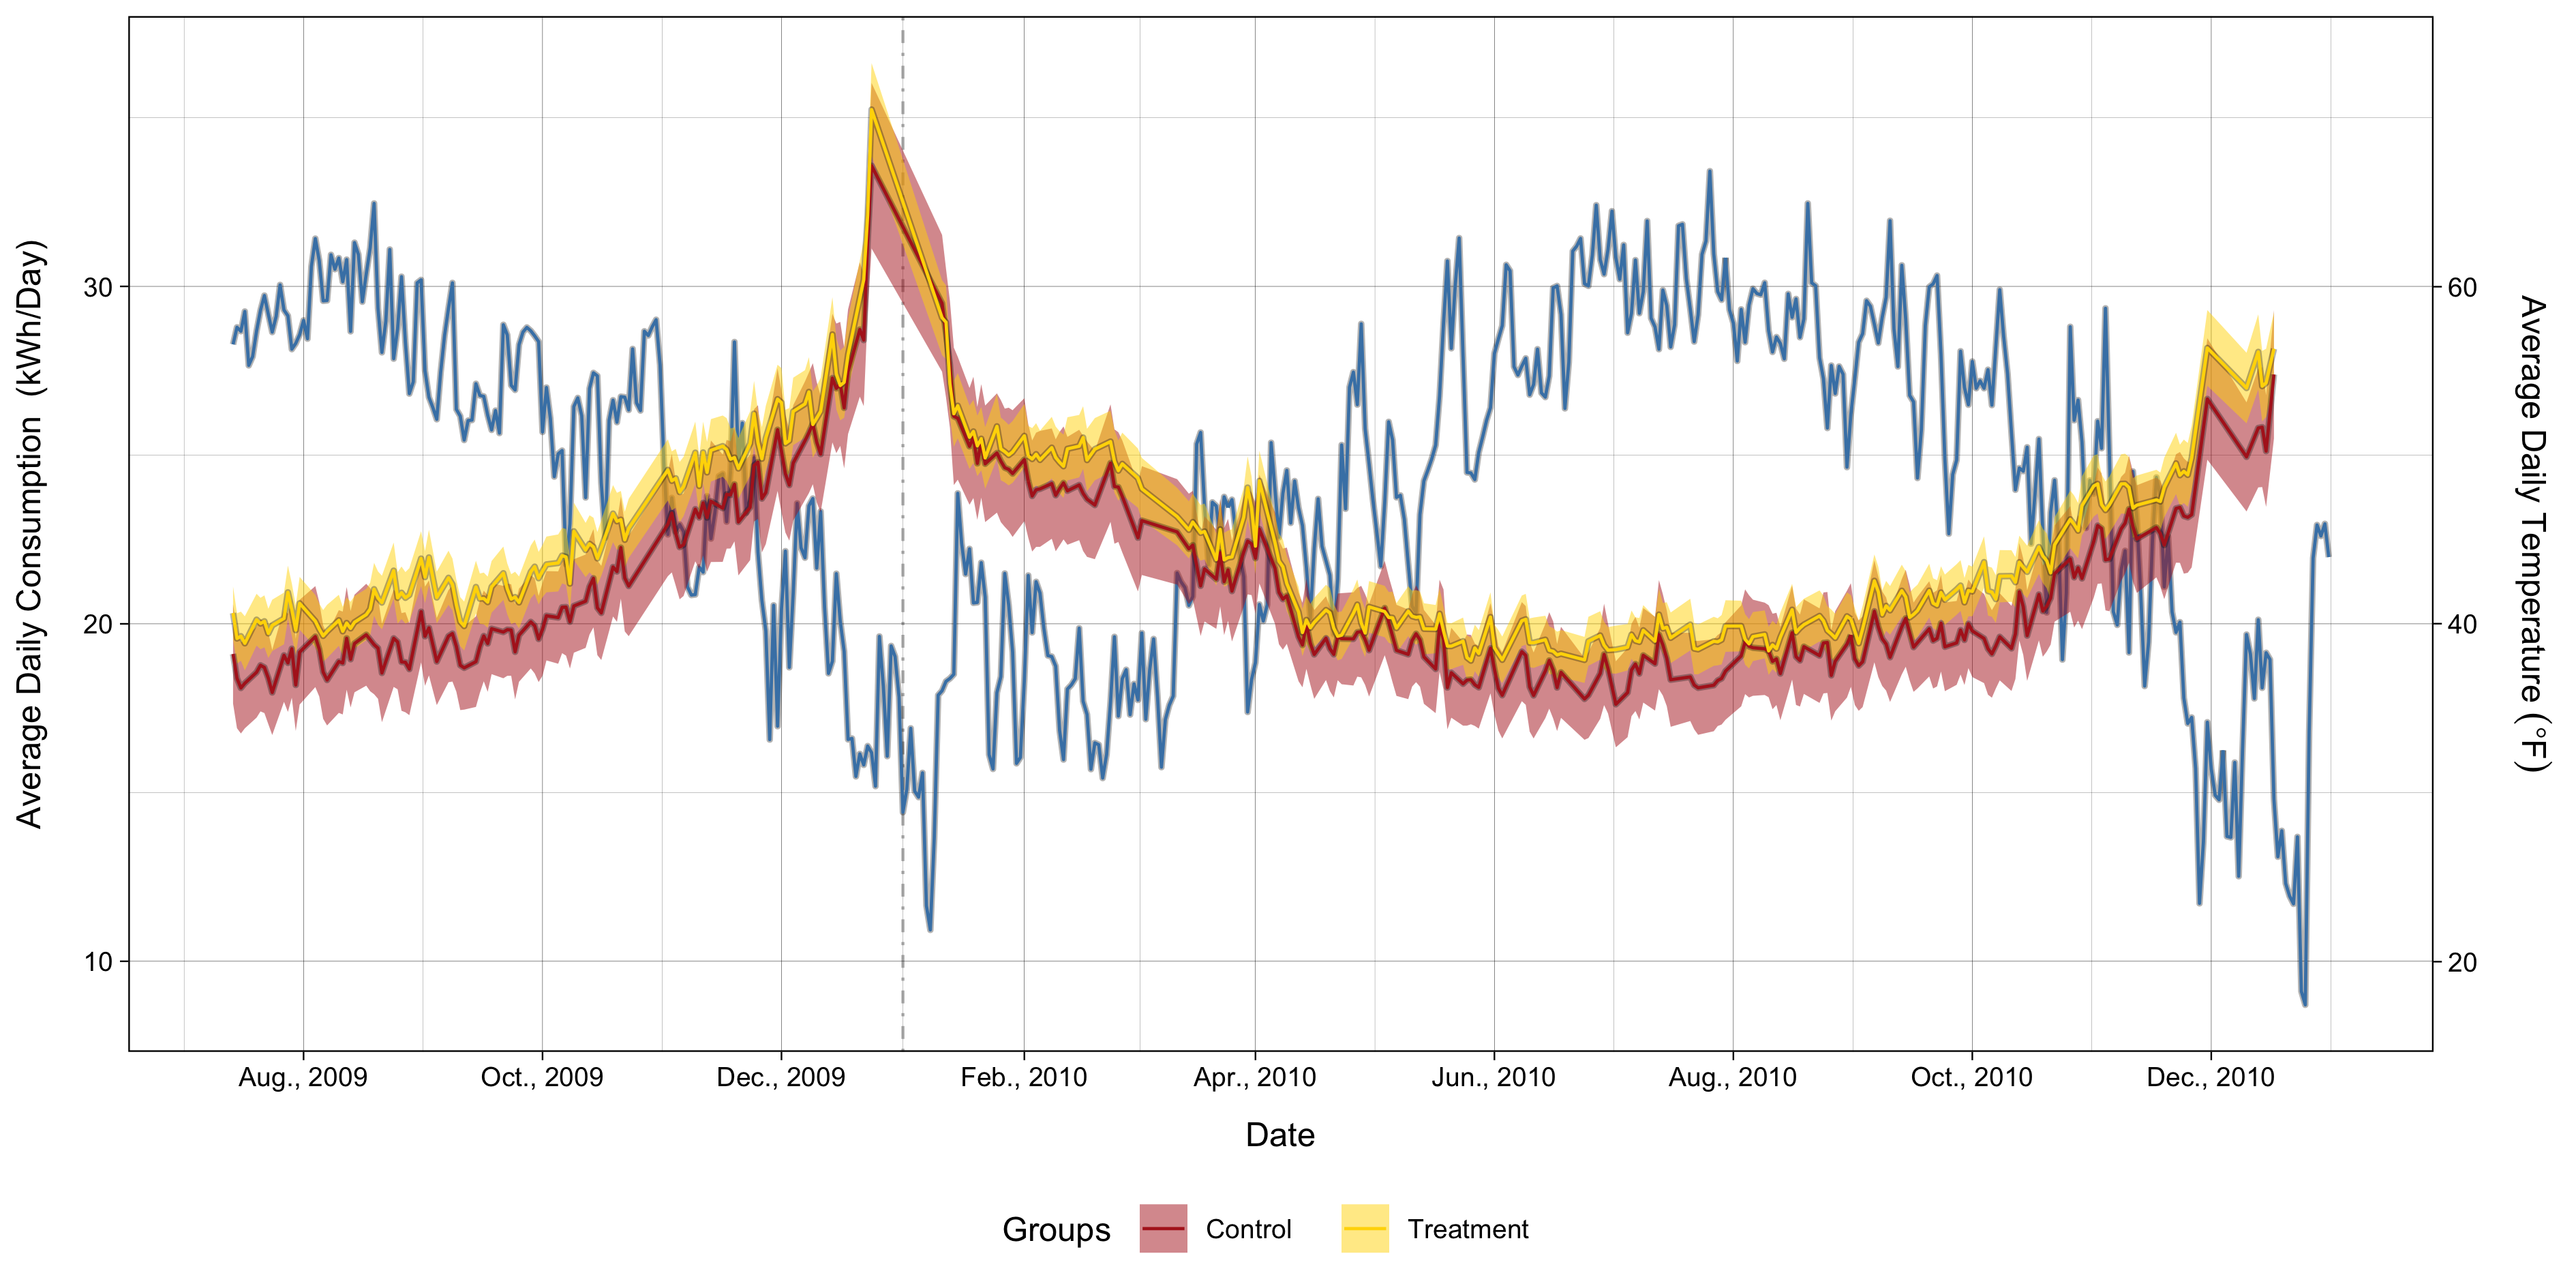
\includegraphics[scale = 0.10]{03_Chapter-2/00A_Figures/Figure_Average-Electricity-Consumption_Average-Daily-Consumption-by-Date.png}
        \caption{Average Daily Electricity Consumption}
        \caption*{
            {\small
            \textit{Note}: The figure depicts, for households that exploit non-electric energy sources for their space and water heating, not only the average daily electricity consumption with 95\% confidence intervals for each group (red and yellow lines) but also the mean daily temperature (blue line). From this figure, it is apparent that household daily electricity consumption is negatively correlated with the average daily temperature. In other words, in Ireland, outdoor temperatures are a crucial driver of within-household electricity consumption.
        }}
        \label{Figure:Average-Daily-Electricity-Consumption}
    \end{figure}
}
Figure \ref{Figure:Average-Daily-Electricity-Consumption} indicates the limitations of focusing on aggregate electricity consumption, as many studies have been doing. The figure clearly shows that aggregate household electricity consumption increases as the weather becomes colder in Ireland. Intuitively, the negative correlation between them can be mainly attributable to for-heating electricity consumption, which strongly depends on outdoor temperatures. It is a fact that aggregate residential electricity consumption also includes another type of electricity consumption: electricity consumption that is irrelevant to temperature variation, such as consumption for lighting. Those two broad categories of electricity consumption could react differently to TOU electricity pricing. Electricity consumption for heating can be transferred to a different time of the day (e.g., from 6 p.m. to 4 p.m. to avoid a higher unit price under the TOU tariff structures). On the other hand, electricity consumption for lighting is time sensitive. Due to the difference in the costs of relocating or changing electricity consumption, it is possible that the two channels of household electricity consumption respond to TOU electricity pricing in different ways. Therefore, using aggregate electricity consumption to examine households' responses to the time-varying price scheme enables me to access only the aggregated response. 

Considering the discussion above, I decompose household electricity consumption into two broad categories---non-temp.-control-driven and temp.-control-driven electricity consumption---and examine how each category of electricity consumption responds to the introduction of the TOU tariff structures. The temperature-control-related electricity consumption here means using electricity to satisfy home heating needs (e.g., to warm up space or water). So, the use of electricity for heating strictly depends on each day's weather conditions, especially temperatures. Naturally, the non-temperature-control-associated electricity consumption makes up the rest. 

I exploit daily Heating Degree Days (HDDs), which imply overall heating needs on a given day, to isolate the temperature-control-driven consumption from aggregate household electricity consumption. Because only aggregate metering data is available from the CER experiment dataset, there is no clue allowing me to classify household electricity consumption into two distinct categories in the dataset. To address this challenge, I presume that the portion of household electricity consumption that fluctuates according to daily HDDs is temperature-control-driven electricity consumption. Therefore, the electricity consumption for temperature-control use is additional consumption that appears only on days with non-zero daily HDDs due to household heating needs.

To break down household responses to the TOU program around the peak rate period, I exploit the following DID-style spline regression model:\footnote{The control group's less percentage changes on freezing days, which are illustrated in Figure (\ref{Figure:Pre-and-Post-Treatment-Household-Average-Daily-Electricity-Consumption}) substantiate the use of the DID-style spline regression model in \ref{Eq:Model-Specification_Breakdown-of-Hourly-Average-Treatment-Effect}.}:
\begin{equation}
\small
\begin{split}
    kWh_{ith} \
    & = \ \beta_{1} HDD_{t} \ + \ \beta_{2} HDD_{t}^{*} \\
    & \hspace{0.7cm} + \ \big( \beta_{3} \ + \ \beta_{4} HDD_{t} \ + \ \beta_{5} HDD_{t}^{*} \big) \mathds{1}[\text{Treatment}]_{i} \\
    & \hspace{0.7cm} + \ \big( \beta_{6} \ + \ \beta_{7} HDD_{t} \ + \ \beta_{8} HDD_{t}^{*} \big) \mathds{1}[\text{Post}]_{t} \\
    & \hspace{0.7cm} + \ \big( \beta_{9} \ + \ \beta_{10} HDD_{t} \ + \ \beta_{11} HDD_{t}^{*} \big) \mathds{1}[\text{Treatment \& Post}]_{it} \ + \ \kappa_{dw} \ + \ \epsilon_{ith} 
\end{split}
\label{Eq:Model-Specification_Breakdown-of-Hourly-Average-Treatment-Effect}
\end{equation}
Like (\ref{Eq:Model-Specification_Hourly-Average-Treatment-Effects}), the dependent variable $kWh_{ith}$ is the electricity consumption by household $i$ on the day $t$ during the hour of the day $h$. In this model, the full set of fixed effects in (\ref{Eq:Model-Specification_Hourly-Average-Treatment-Effects}) has been superseded by two indicator variables---the first indicator variable $\mathbb{1}[\text{Treatment}]_{i}$ has the value of 1 if household $i$ is assigned to the treatment group, and the second indicator variable $\mathbb{1}[\text{Post}]_{t}$ equals 1 when the day $t$ is in the treatment period. Although using the fixed effects as in (\ref{Eq:Model-Specification_Hourly-Average-Treatment-Effects}) does not affect the treatment effects of interests, which is expected given the randomization, replacing them with the indicator variables allows for the interpretation of the average consumption by the treatment group to be more straightforward.\footnote{Added indicator variables instead of various fixed effects also enables an easier graphical summary of the regression results.} The model also includes interaction terms between HDD-relevant terms and those indicator variables. In the econometric model, $HDD_{t}$ means the daily heating degree days on the day $t$. And $HDD_{t}^{*}$, which is required to introduce nonlinearity in HDD-associated response to TOU pricing, is mathematically defined as follows:
\begin{equation}
\small
HDD_{t}^{*} \ = \ (HDD_{t} - Knot) \ \times \ \mathbb{1}[HDD_{t} > Knot],
\end{equation}
where $Knot$ is a reference value at which the slope of the predicted line starts to change. For $Knot$, I utilize the value of ten in the following regression analysis because the median values of daily HDDs in the baseline and treatment periods are ten. The term $\kappa_{dw}$ is day-of-week-by-half-hourly-time-window fixed effects. 

The primary coefficients of interest in (\ref{Eq:Model-Specification_Breakdown-of-Hourly-Average-Treatment-Effect}) are $\beta_{9}$, $\beta_{10}$, and $\beta_{11}$. The three coefficients show how much electricity consumption changes in the households assigned to the treatment group changed after implementing the TOU program compared to those in the control group. To be specific, $\beta_{9}$ demonstrates the change in residential electricity consumption for non-temperature-control use. Both $\beta_{10}$ and $\beta_{11}$ collectively represent the change in the amount of electricity consumed to meet household heating needs at given daily HDDs. 

\afterpage{
    \begin{figure}[t!]
        \centering
        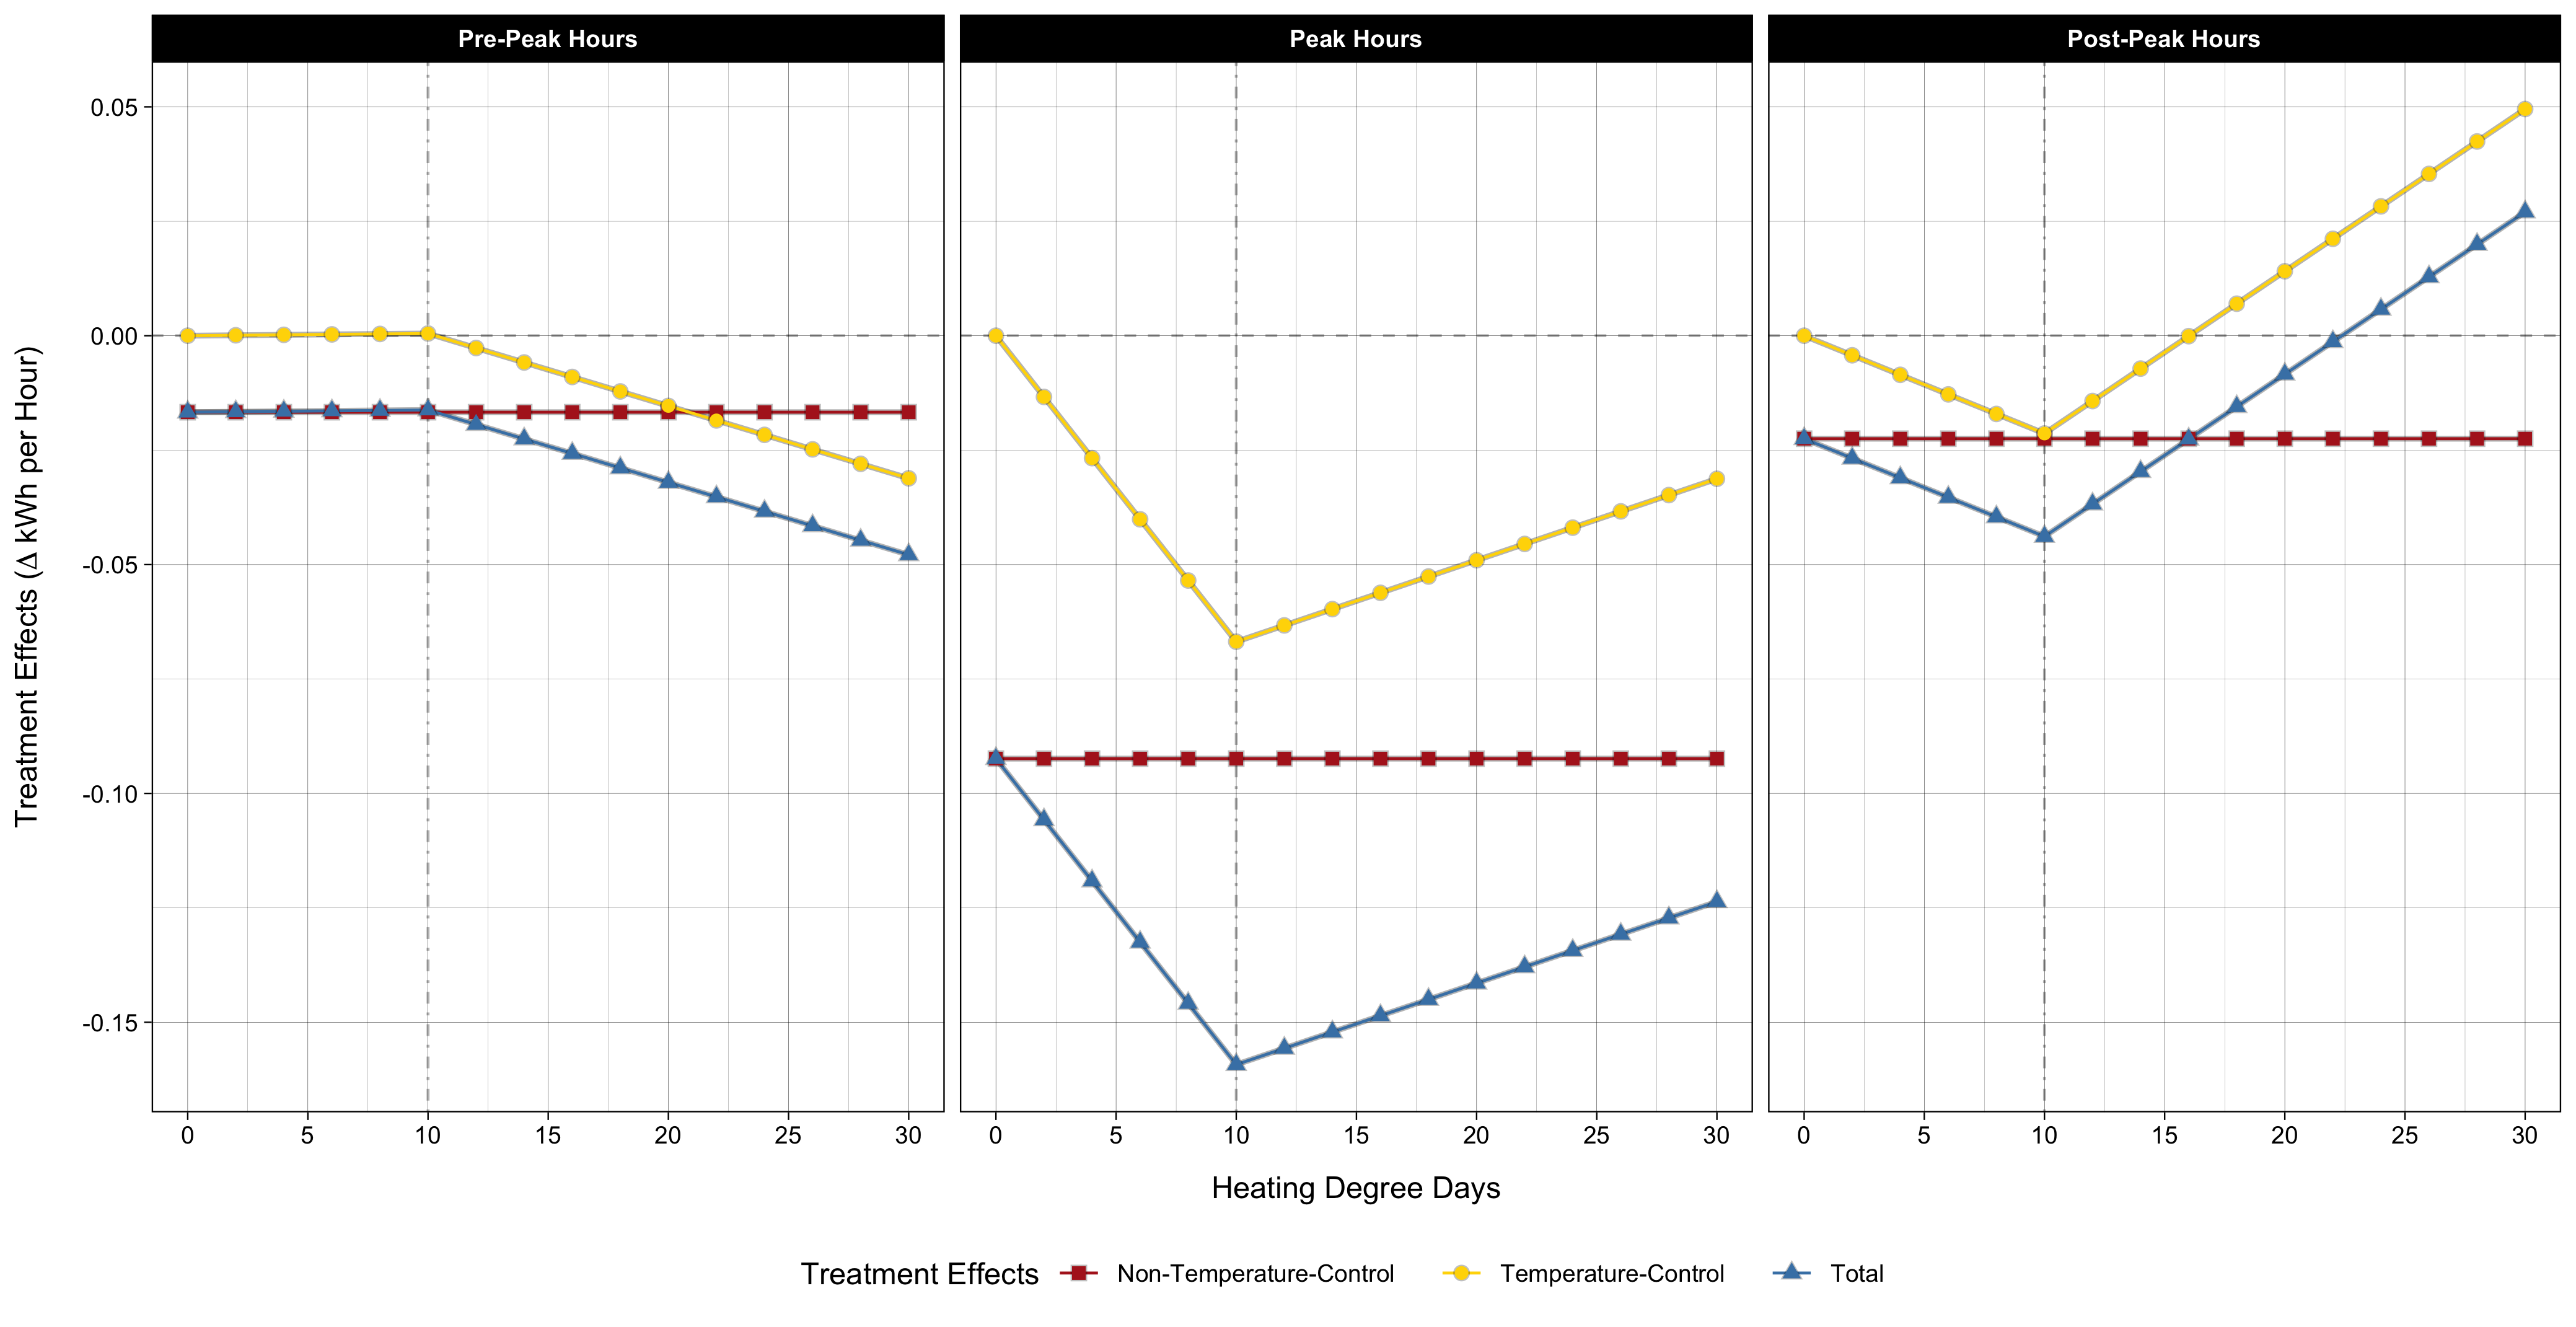
\includegraphics[scale = 0.105]{03_Chapter-2/00A_Figures/Figure_Breakdown-of-Hourly-ATEs_For-Different-Intervals_All_Knot-10.png}
        \caption{Breakdown of Hourly Average Treatment Effects}
        \caption*{
            {\small
            \textit{Note}: This figure is a graphical summary of the regression results. The order of panes corresponds to that of columns. As clearly illustrated, each two-hour interval shows distinct evolving patterns of two broad categories of household electricity consumption. The changes in non-temperature-control-driven household electricity consumption are straight lines because they are independent of outdoor temperature variation. On the other hand, the changes in temperature-control-associated residential electricity consumption are a nonlinear function of daily HDDs.
        }}
        \label{Figure:Breakdown-of-Hourly-ATEs-in-the-Peak-Rate-Period}
    \end{figure}
}
Using the point estimates of the three coefficients of interest, I graphically summarize the predicted change in each of the two channels of electricity consumption in Figure \ref{Figure:Breakdown-of-Hourly-ATEs-in-the-Peak-Rate-Period}. Regarding the change in electricity consumption for non-temperature-control use, the table and figure clearly show that the treated households significantly reduced their consumption when subject to peak-hour prices (i.e., in the peak rate period). Their non-temperature-control-driven electricity consumption also decreased in the pre- and post-peak periods, albeit noisy and relatively smaller in magnitude than the peak-hour changes. 

The change in temperature-control-associated electricity consumption occurred as well in all three two-hour periods, but its evolving pattern over daily HDDs was quite different in each period. Specifically, the impact of TOU pricing on residential electricity consumption for heating was U-shaped in the peak rate period. In contrast, in the hours before and after the peak period, the TOU intervention altered the electricity use for heating only on the coldest days (i.e., only when daily HDDs were sufficiently large). In other words, from the figure, it is evident that the change originating from temperature-control-related electricity consumption was a nonlinear function of daily HDDs in all three periods.

Specification (\ref{Eq:Model-Specification_Breakdown-of-Hourly-Average-Treatment-Effect}) is also utilized to examine, for the peak rate period, the relationship between the degree of a price increase in that period and the change in electricity consumption. On the whole, the reduction stemming from electricity demand for non-temperature-control use tends to be proportional to the size of price growth in peak hours, even though the point estimate for Tariff Group C is an exception. Therefore, the marginally diminishing effects of TOU pricing, discussed in \cite{Peaking-Interest:How-Awareness-Drives-the-Effectiveness-of-Time-of-Use-Electricity-Pricing_Prest_2020}, seem not to be championed by my point estimates. To be specific, while the aggregate electricity consumption during the peak rate period does not sensibly respond to incremental changes in the peak-hour price, the amount of electricity used for non-temperature-control purposes in the peak rate period does respond meaningfully to the marginal changes in the peak price. And the two estimates associated with temperature-control-driven electricity consumption (i.e., $\hat{\beta}_{10}$ and $\hat{\beta}_{11}$) are statistically significant only for the case of the smallest price increase.\footnote{In case of Tariff Group D, only $\hat{\beta}_{11}$ is statistically significant.} 

Altogether, those results imply two interesting points. First, the two distinct types of electricity consumption showed widely different responses to TOU prices in all three periods of two hours. Second, the measured reductions in non-temperature-control-related electricity consumption seem highly sensitive to the magnitude of a price increase in the peak rate period. Inspired by those implications, I formulate the resulting variations in household electricity consumption as a linear function of the magnitude of a rate change in peak-demand hours in the following section.


\subsubsection{Household Responses as a Linear Function of Price Changes}
\label{Sub-subsection:Household-Responses-as-a-Linear-Function-of-Price-Changes}
To fully understand how residential consumers adjust their consumption behavior as a set of reactions to the price changes under the TOU program, it is necessary to explicitly examine, for each of the three periods (i.e., the pre-peak, peak, and post-peak periods), the relationship between the size of a price increase in the peak rate period and the changes in the two distinct categories of household electricity consumption. For that reason, I quantitatively determine the relationship by utilizing the following econometric model:
\begin{equation}
\small
\begin{split}
    kWh_{ith} \ 
%    & = \ \beta_{1} HDD_{t} \ + \ \beta_{2} HDD_{t}^{*} \\
%    & \hspace{0.7cm} + \ \beta_{3} \mathds{1}[\text{Treatment}]_{i} \ + \ \beta_{4} \mathds{1}[\text{Treatment}]_{i} \Delta RC_{i} \\
%    & \hspace{0.7cm} + \ \beta_{5} HDD_{t} \mathds{1}[\text{Treatment}]_{i} \ + \ \beta_{6} HDD_{t} \mathds{1}[\text{Treatment}]_{i} \Delta RC_{i} \\
%    & \hspace{0.7cm} + \ \beta_{7} HDD_{t}^{*} \mathds{1}[\text{Treatment}]_{i} \ + \ \beta_{8} HDD_{t}^{*} \mathds{1}[\text{Treatment}]_{i} \Delta RC_{i} \\
%    & \hspace{0.7cm} + \ \beta_{9} \mathds{1}[\text{Post}]_{t} \ + \ \beta_{10} HDD_{t} \mathds{1}[\text{Post}]_{t} \ + \ \beta_{11} HDD_{t}^{*} \mathds{1}[\text{Post}]_{t} \\
%    & \hspace{0.7cm} + \ \beta_{12} \mathds{1}[\text{Treatment \& Post}]_{it} \ + \ \beta_{13} \mathds{1}[\text{Treatment \& Post}]_{i} \Delta RC_{i} \\
%    & \hspace{0.7cm} + \ \beta_{14} HDD_{t} \mathds{1}[\text{Treatment \& Post}]_{it} \ + \ \beta_{15} HDD_{t} \mathds{1}[\text{Treatment \& Post}]_{i} \Delta RC_{i} \\
%    & \hspace{0.7cm} + \ \beta_{16} HDD_{t}^{*} \mathds{1}[\text{Treatment \& Post}]_{it} \ + \ \beta_{17} HDD_{t}^{*} \mathds{1}[\text{Treatment \& Post}]_{i} \Delta RC_{i} \ + \ \alpha_{dw} \ + \ \epsilon_{ith}
%    & = \ \beta_{1} HDD_{t} \ + \ \beta_{2} HDD_{t}^{*} \\
%    & \hspace{0.7cm} + \ \big( \beta_{3} \ + \ \beta_{4} HDD_{t} \ + \ \beta_{5} HDD_{t}^{*} \big) \mathds{1}[\text{Treatment}]_{i} \\
%    & \hspace{0.7cm} + \ \big( \beta_{6} \ + \ \beta_{7} HDD_{t} \ + \ \beta_{8} HDD_{t}^{*} \big) \mathds{1}[\text{Treatment}]_{i} \Delta RC_{i} \\
%    & \hspace{0.7cm} + \ \big( \beta_{9} \ + \ \beta_{10} HDD_{t} \ + \ \beta_{11} HDD_{t}^{*} \big) \mathds{1}[\text{Post}]_{t} \\
%    & \hspace{0.7cm} + \ \big( \beta_{12} \ + \ \beta_{13} HDD_{t} \ + \ \beta_{14} HDD_{t}^{*} \big) \mathds{1}[\text{Treatment \& Post}]_{it} \\
%    & \hspace{0.7cm} + \ \big( \beta_{15} \ + \ \beta_{16} HDD_{t} \ + \ \beta_{17} HDD_{t}^{*} \big) \mathds{1}[\text{Treatment \& Post}]_{i} \Delta RC_{i} \\
%    & \hspace{0.7cm} + \ \alpha_{dw} \ + \ \epsilon_{ith}
    & = \ \beta_{1} HDD_{t} \ + \ \beta_{2} HDD_{t}^{*} \\
    & \hspace{0.7cm} + \ \big( \beta_{3} \ + \ \beta_{4} HDD_{t} \ + \ \beta_{5} HDD_{t}^{*} \big) \mathds{1}[\text{Treatment}]_{i} \\
    & \hspace{0.7cm} + \ \big( \beta_{6} \ + \ \beta_{7} HDD_{t} \ + \ \beta_{8} HDD_{t}^{*} \big) \mathds{1}[\text{Treatment}]_{i} \Delta PC_{i} \\
    & \hspace{0.7cm} + \ \big( \beta_{9} \ + \ \beta_{10} HDD_{t} \ + \ \beta_{11} HDD_{t}^{*} \big) \mathds{1}[\text{Post}]_{t} \\
    & \hspace{0.7cm} + \ \big( \beta_{12} \ + \ \beta_{13} HDD_{t} \ + \ \beta_{14} HDD_{t}^{*} \big) \mathds{1}[\text{Treatment \& Post}]_{it} \\
    & \hspace{0.7cm} + \ \big( \beta_{15} \ + \ \beta_{16} HDD_{t} \ + \ \beta_{17} HDD_{t}^{*} \big) \mathds{1}[\text{Treatment \& Post}]_{i} \Delta PC_{i} \ + \ \kappa_{dw} \ + \ \epsilon_{ith}
\end{split}
\label{Eq:Model-Specification_Breakdown-of-Hourly-Average-Treatment-Effect-as-a-Linear-Function-of-Price-Changes}
\end{equation}
The model is the same with (\ref{Eq:Model-Specification_Breakdown-of-Hourly-Average-Treatment-Effect}) except for interaction terms between treatment-status-relevant indicator variables (i.e., $\mathds{1}[\text{Treatment}]_{i}$ and $\mathds{1}[\text{Treatment \& Post}]_{it}$) and $\Delta PC_{i}$, where $\Delta PC_{i}$ is the difference between the peak-hour prices in the treatment period and the flat rate in the baseline period. The coefficients of the second interaction term (i.e., $\beta_{15}$, $\beta_{16}$, and $\beta_{17}$) capture the impacts of deploying TOU tariffs on household electricity consumption as a linear function of the degree of a peak-demand-hour price change. 

The estimates of the six coefficients of interest (i.e., from $\beta_{12}$ to $\beta_{17}$) presented in Table \ref{Table:Hourly-ATEs-as-a-Linear-Function-of-Peak-Rate-Period-Price-Changes_Coefficients-of-Interest-only} are summarized graphically in Figure \ref{Figure:Treatment-Effects-as-a-Linear-Function-of-Price-Changes-in-the-Peak-Rate-Period}, which is extensively exploited throughout this paper. And this figure, showing the estimated treatment effects for the two consumption channels and the sum of the treatment effects in each of the three intervals, re-confirms the finding of peak-rate-period price increases' diminishing returns in \cite{Peaking-Interest:How-Awareness-Drives-the-Effectiveness-of-Time-of-Use-Electricity-Pricing_Prest_2020}. 

In the peak rate period, the reduction in non-temperature-control-associated electricity consumption increased as the magnitude of a peak-hour price increase grew (see the panel in the first row of the second column of Figure \ref{Figure:Treatment-Effects-as-a-Linear-Function-of-Price-Changes-in-the-Peak-Rate-Period}). On the contrary, at given daily HDDs, the reduction in temperature-control-related electricity consumption weakly moved towards zero as the size of a peak-demand-hour tariff escalation increased (see the panel in the second row of the second column of Figure \ref{Figure:Treatment-Effects-as-a-Linear-Function-of-Price-Changes-in-the-Peak-Rate-Period}). As well illustrated in the panel in the third row of the second column of Figure \ref{Figure:Treatment-Effects-as-a-Linear-Function-of-Price-Changes-in-the-Peak-Rate-Period}, for a given value of daily HDDs, the differences in treatment effect across the level of price growth are seemingly dampened when the estimated treatment effects from two distinct categories of electricity consumption are aggregated due to the opposite response to peak-hour price increases in the two consumption categories.\footnote{The last row of Figure \ref{Figure:Treatment-Effects-as-a-Linear-Function-of-Price-Changes-in-the-Peak-Rate-Period} shows the sum of the first and second rows.} Indeed, this empirical result is consistent with the finding discussed in the paper that a higher price results in a larger diminution in electricity demand, while additional gains diminish in the peak interval. 

In the two-hour interval before the peak rate period, the two types of residential electricity consumption continue to respond differently to the peak price for given daily HDDs, but the pattern is now switched. The pre-peak period exhibits a more significant reduction in non-temperature-control-driven electricity consumption for a more minor change in peak-hour price (see the panel in the first row of the first column of Figure \ref{Figure:Treatment-Effects-as-a-Linear-Function-of-Price-Changes-in-the-Peak-Rate-Period}). By contrast, the larger the magnitude of a peak-rate-period price change, the wider the diminution in temperature-control-related electricity consumption during the pre-peak period (see the panel in the second row of the first column of Figure \ref{Figure:Treatment-Effects-as-a-Linear-Function-of-Price-Changes-in-the-Peak-Rate-Period}). For the same reason as in the peak period, the aggregate treatment effects of the TOU tariffs described in the last row of the first column of Figure \ref{Figure:Treatment-Effects-as-a-Linear-Function-of-Price-Changes-in-the-Peak-Rate-Period} are seemingly less sensitive to peak-hour prices. Note that regarding electricity consumption for heating during the pre-peak period, TOU electricity pricing played a role only when household heating needs were sufficiently high.

Irish residential consumers adjusted their electricity consumption behavior during the post-peak period as well. As in the pre-peak period, consumption changes stemming from non-temperature-control-related electricity use increased as the size of a peak-demand-hour rate change diminished (see the panel in the first row of the third column of Figure \ref{Figure:Treatment-Effects-as-a-Linear-Function-of-Price-Changes-in-the-Peak-Rate-Period}). The TOU-price-induced change in temperature-control-driven electricity consumption evolved over daily HDDs somewhat complicatedly. Though depending on the magnitude of a peak-hour price increase, TOU tariffs reduced household electricity consumption for heating on Ireland's typical winter days in that period. Interestingly, the CER TOU program provoked additional heating-related consumption during the post-peak period on extremely cold days in Ireland. In addition, as the level of peak-demand-hour price alteration grew, the profile of measured treatment effect for temperature-control-associated consumption moved downward. Consequently, a higher price increase in the peak rate period resulted in a more significant reduction in electricity consumption for heating when heating demands were lower, while a smaller addition to electricity consumption for heating on cold winter days (see the panel in the second row of the third column of Figure \ref{Figure:Treatment-Effects-as-a-Linear-Function-of-Price-Changes-in-the-Peak-Rate-Period}). Altogether, as shown in the last row of the third column of Figure \ref{Figure:Treatment-Effects-as-a-Linear-Function-of-Price-Changes-in-the-Peak-Rate-Period}, the aggregate treatment effects of the TOU program in the post-peak period are superficially moderated because of households' opposite responses to peak-demand-hour price increases in the two distinct channels of electricity consumption.  

In summary, under TOU electricity pricing, the degree of a price change in peak-demand hours, not just its existence, still matters to residential consumers' electricity consumption. The empirical results above suggest that the opposite directional changes in the two channels of electricity consumption make Irish households appear insensitive to the time-varying price structure. In other words, their high sensitivity to TOU prices is revealed only when their electricity consumption is disaggregated. Together with the empirical findings in previous sections, the results imply that three simultaneously interacting factors govern the dynamics of residential electricity consumption under TOU pricing: the timing when electricity is consumed, daily HDDs, and the magnitude of price increase in the peak rate period.  



\subsection{Dynamics of Household Electricity Consumption under TOU Pricing}
\label{Subsection:Dynamics-of-Household-Electricity-Consumption-under-Time-Of-Use-Electricity-Pricing}

%The preceding results from my empirical analysis highlight that households were quite responsive to incremental changes in the peak-demand-hour price. As the peak-hour price increased compared to the flat rate, non-temperature-control-related electricity consumption continued to decline in the peak rate period. In contrast, temperature-control-driven consumption did indeed fall, but these reductions in residential electricity consumption occurred outside of the peak rate period (i.e., in the pre- and post-peak periods). In this section, I will further examine what can drive these different patterns in the responses to TOU prices. 

\subsubsection{Mechanism: Load-shedding vs. Load-shifting}
\label{Sub-subsection:Mechanism}
Examining participating households' electricity consumption, following a time sequence from the pre-peak to the post-peak period, facilitates a complete understanding of how they adapted to the TOU tariff structures in the CER experiment. Intuitively, residential consumers can respond to TOU tariffs by conserving their electricity consumption during the peak-demand hours, leading to an overall reduction in their demand for electricity. Instead of reducing their electricity consumption, they can shift it to off-peak hours so as not to be subject to the peak rate as much as possible. In this case, the level of their net electricity consumption in a day is maintained. Of course, those two ways of responding to time-varying price structures can co-occur. Because those two ways reshape load curves not only in the peak rate period but also in the hours surrounding that period, it will be natural to examine the impact of the TOU program on household electricity consumption from a time-moving perspective in order to grasp the whole dynamics of households' behavioral changes. In the following paragraphs, I will provide interpretations of the changes in households' consumption behavior, which are observed in my empirical analysis. 

Regarding residential electricity demand for non-temperature-control uses, the leading reaction of the treated households to the TOU tariffs was to reduce their consumption in and near the peak rate period. According to my regression results summarized in Figure \ref{Figure:Treatment-Effects-as-a-Linear-Function-of-Price-Changes-in-the-Peak-Rate-Period}, in the peak rate period, the reduction in non-temperature-control-related electricity consumption increased as the magnitude of the price change in that period under the TOU program grew. Non-temperature-control-driven electricity consumption in the pre- and post-peak periods showed a weak but opposite variation---i.e., the reduction originating from households' non-for-heating consumption moved towards zero as the degree of the price increase in the peak rate period became larger. In the case of Tariff Group A, although there was almost zero price variation relative to the flat rate (i.e., only 0.1 cents per kWh) in the pre- and post-peak periods, the amount of the diminution in non-temperature-control-related electricity consumption for that group was nearly the same in all three periods. Meanwhile, despite more sizable price decreases, the remaining tariff groups also conserved, or at least sustained, their consumption for non-temperature-control uses in both surrounding periods. In other words, my empirical results reveal that reductions in households' non-for-heating electricity consumption spilled over into non-peak periods (i.e., the pre- and post-peak periods). 

A remarkable point with respect to the spillovers to non-peak hours, suggesting households' behavioral changes related to non-temperature-control-driven electricity consumption in the pre- and post-peak periods, is that they seemed to relocate a part of their not-for-heating electricity consumption during peak hours to those two periods. As described in Figure \ref{Figure:Time-Of-Use-Pricing-Structures}, there were price drops in the hours before and after the peak rate period. Furthermore, for marginal electricity consumption, because the tariff group that paid the highest price in the peak rate period (i.e., Tariff Group D) paid the lowest price in the surrounding hours, the households in that group were more incentivized to move their peak-hour electricity consumption to off-peak hours. Hence, the phenomenon that the reduction in not-for-heating electricity consumption in the surrounding periods declined as the magnitude of the peak-rate-period price change increased is well explained by combining the load-shedding with the load-shifting, which was motivated by the monetary incentive from the price differences between the peak and off-peak periods. As shown in Figure \ref{Figure:Treatment-Effects-as-a-Linear-Function-of-Price-Changes-in-the-Peak-Rate-Period}, the relocation-associated consumption change, in general, did not fully outweigh the conservation-relevant one in both periods. 

Taken together, with respect to non-temperature-control-driven electricity consumption, the households assigned to the treatment group responded to the TOU program via load-shedding as primary and load-shifting as secondary reactions. Interestingly, the total non-temperature-control-relevant reduction in and near the peak rate period, which is depicted in the fourth column of the first row in Figure \ref{Figure:Treatment-Effects-as-a-Linear-Function-of-Price-Changes-in-the-Peak-Rate-Period}, did not vary with the level of a peak-hour price increase. This outcome might reflect households' limited capability not only to identify possible sources of reducing their electricity consumption but also to realize lower consumption from the sources. 

With respect to temperature-control-related household electricity consumption, Figure \ref{Figure:Treatment-Effects-as-a-Linear-Function-of-Price-Changes-in-the-Peak-Rate-Period} depicts that the program caused a reduction in for-heating electricity use during the peak rate period, especially around typical values of daily HDDs during winter in Ireland. Interestingly, although statistically insignificant, the smaller the magnitude of the peak-demand-hour price change increase, the larger the induced reduction in temperature-control-related consumption in the peak period. That is, the change in for-heating electricity consumption seems to violate the law of demand. As discussed above, the households assigned to Tariff Group D had the highest incentive to relocate their peak-hour electricity consumption to non-peak hours surrounding the peak-demand hours due to the largest across-period price difference. Therefore, the reduction in electricity consumption for heating in the pre-peak period, which occurred only on days with heavy heating needs, cannot be explained as a consequence of either the price decrease in that period or load-shifting. In other words, regarding temperature-control-driven household electricity consumption, as did in the peak rate period, the price signals did not function well in the pre-peak period. In the post-peak period, high daily HDDs incurred additional electricity consumption for heating after introducing TOU tariffs. The degree of the additional consumption, however, also cannot be justified by the price signals for the same reasons as in the pre-peak period.\footnote{The estimated changes in temperature-control-related electricity consumption with respect to peak-demand-hour price variation for the peak and post-peak periods, presented in Figure \ref{Figure:Treatment-Effects-as-a-Linear-Function-of-Price-Changes-in-the-Peak-Rate-Period}, seem rather to imply that the degree of load-shifting diminished as the financial incentive, measured by the price difference between the two periods, increased.} And the amount of the additional consumption was generally not large enough to fully offset, for given heating needs in a day, the reduction in the preceding periods. In Section \ref{Sub-subsection:Household-Electricity-Consumption-for-Heating-in-a-Time-Line}, I will discuss a possible explanation for the consumption behavior not backed by the price signals. 


\subsubsection{Household Electricity Consumption for Heating in a Time Line}
\label{Sub-subsection:Household-Electricity-Consumption-for-Heating-in-a-Time-Line}
From Figure \ref{Figure:Treatment-Effects-as-a-Linear-Function-of-Price-Changes-in-the-Peak-Rate-Period}, examining the curves that illustrate the change in temperature-control-associated electricity consumption for three consecutive periods simultaneously, but taking account of their time sequence, suggests a significant implication of the effectiveness of the TOU prices in the peak rate period. According to the figure, as the degree of peak-hour price escalation increased, the temperature-control-related consumption reduction in the pre-peak period expanded, while those in the peak period decreased gradually. Altogether, it is likely that a larger pre-adjustment leads to a smaller reduction in electricity demand for heating during peak-demand hours, which in turn seems to result in limited additional consumption during the following post-peak period. Compared to the case that a household does not reduce for-heating electricity consumption during the pre-peak period, consuming more for-heating electricity during peak hours seems necessary to prevent indoor temperatures from falling too much or persisting at a low level when the household significantly reduces its temperature-control-driven consumption during the pre-peak period.\footnote{This interpretation is in line with the concept ``discomfort'' in \cite{Smart-Thermoststs-Automation-and-Time-Varying-Prices_Blonz-et-al_2021}. See Section 3.4 in the paper.} In addition, the household will have less incentive to increase its electricity consumption for heating during post-peak hours since its room temperatures will be higher than if it were to reduce its electricity consumption for heating during peak hours considerably. In light of the fact that TOU tariffs are intended to conserve electricity consumption during peak-demand hours, it is reasonable to conclude that a lower reduction in peak hours due to a too large pre-adjustment results in a deterioration in the performance of the TOU tariffs. 

As discussed in detail, under the TOU program, households' adjustments to their behavior for temperature-control-driven electricity consumption during the pre-peak hours seem to determine the degree of a reduction in that use of electricity during the following period (i.e., during the peak rate period) in lieu of price signals. In Figure \ref{Figure:Treatment-Effects-as-a-Linear-Function-of-Price-Changes-in-the-Peak-Rate-Period}, the gap in the temperature-control-related treatment effect at given daily HDDs between the lowest and the highest peak-hour rate changes, therefore, might be understood as potentially attainable gains when the pre-adjustments are suppressed. This explanation motivates the necessity of adopting home automation technologies, like Programmable Communicating Thermostats (PCTs), to restrict such adjustments only to the peak rate period. Considering the fact that households generally set a target temperature instead of micromanaging their heating devices according to ever-changing outdoor temperatures, PCTs with recommended default settings for temperature-control-associated use of electricity are highly likely to contribute to minimizing their behavioral changes prior to the peak rate period.\footnote{\cite{Default-Effects-and-Follow-on-Behavior_Evidence-from-an-Electricity-Pricing-Program_Fowlie-et-al_2021} examines default effects in a randomized controlled trial, in which the participants assigned to the control group defaulted into a residential electricity pricing program. Default effects have been studied in a range of settings, such as organ donation \citep{Medicine_Do-Defaults-Save-Lives_Johnson-and-Goldstein_2003, The-Impact-of-Presumed-Consent-Legislation-on-Cadaveric-Organ-Donoation_Abadie-and-Gay_2006}, car insurance \citep{Framing-Probability-Distortions-and-Insurance-Decisions_Johnson-et-al_1993}, and participation in retirement savings plans \citep{Status-Quo-Bias-in-Decision-Making_Samuelson-and-Zeckhauser_1988, The-Power-of-Suggestion_Madrian-and-Shea_2001, For-Better-or-For-Worse_Choi-et-al_2019}.} Moreover, the additional gains realized by utilizing the automated instruments provide legitimacy for the ongoing SEAI-offering Home Energy Grants, in which heating controls are an essential part.\footnote{Sustainable Energy Authority of Ireland (SEAI) is Ireland's national sustainable energy authority whose goal is to promote and assist the development of sustainable energy in Ireland. Detailed information about Home Energy Grants is available at \url{https://www.seai.ie/grants/research-funding/}.} 
